\documentclass[text05.tex]{subfiles}
\begin{document}
\subsection{アナログ入力そうち}\label{analog_in}
\subsubsection{\ruby{感圧}{かん|あつ}センサー}\label{touch}
\begin{table}[H]
  \begin{widerrows}
    \begin{tabular}{|p{\colF}|p{\colG}|}	\hline
    \ruby{名称}{めい|しょう} & \ruby{感圧}{かん|あつ}センサー（かんあつせんさー）\\ \hline
    \ruby{接続箇所}{せつ|ぞく|か|しょ} & アナログコネクタ (3pin)\\ \hline
    \ruby{機能概要}{き|のう|がい|よう} & \ruby{圧力}{あつ|りょく}を\ruby{測定}{そく|てい}する\\ \hline
    \end{tabular}
  \end{widerrows} 
\end{table}

\begin{table}[H]
  \begin{widerrows}
    \begin{tabular}{|p{\colF}|p{\colG}|}	\hline
    サンプルコードの場所 & 05/anain.hsp\\ \hline
    raspiへの入力 & 0～1023の\ruby{値}{あたい}で\ruby{圧力}{あつ|りょく}を\ruby{測定}{そく|てい}します。\ruby{圧力}{あつ|りょく}がかかるほど\ruby{値}{あたい}が小さくなります。\\ \hline
    raspiへの入力方法 & val = \adcget(ピン番号, チャンネル番号)\\ \hline
    raspiからの出力 & なし\\ \hline
    raspiからの出力方法 & なし\\ \hline
    \end{tabular}
  \end{widerrows} 
\end{table}

\begin{table}[H]
  \begin{widerrows}
    \begin{tabular}{|p{\colF}|p{\colG}|} \hline
    使い道 & \ruby{圧力}{あつ|りょく}を調べる、重さをはかる。\\ \hline
    \ruby{注意事項}{ちゅう|い|じ|こう} & \ruby{圧力}{あつ|りょく}を感知する部分を折り曲げないように注意。\\ \hline
    \ruby{補足}{ほ|そく} & なし\\ \hline
    \end{tabular}
  \end{widerrows} 
\end{table}

\begin{figure}[H]
  \begin{widerrows}
    \begin{tabular}{|p{\colH}|p{\colI}|p{\colH}|p{\colI}|} \hline
    外観 & 
    \begin{minipage}[t]{\linewidth}
      \smallskip
        \centering
        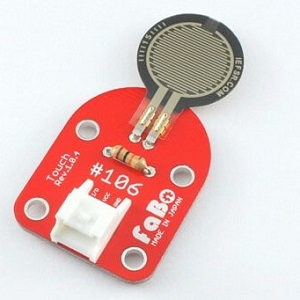
\includegraphics[width=0.5\linewidth]{../../asset/image/text05-img021.jpg}
        \caption{\ruby{感圧}{かん|あつ}センサー}
        \smallskip
      \end{minipage} &
      回路記号 & 
      \begin{minipage}[t]{\linewidth}
      \smallskip
        \centering
        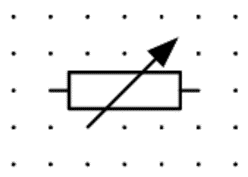
\includegraphics[width=0.5\linewidth]{../../asset/image/text05-img049.png}
        \caption{\ruby{感圧}{かん|あつ}センサーの回路図}
        \smallskip
      \end{minipage}\\ \hline
    \end{tabular}
  \end{widerrows} 
\end{figure}
\end{document}
